\documentclass{beamer}
\usepackage{beamerthemeshadow}


\begin{document}
\title{Soutenance mi-parcours PFE}  
\author{Timothée Schmoderer}
\date{\today} 

\frame{\titlepage} 

\frame{\frametitle{Au menu}\tableofcontents} 


\section{Introduction} 
\frame{\frametitle{Introduction} 
\begin{itemize}
\item Gaspard Monge 1871 - \emph{Mémoire sur la théorie des déblais et des remblais}
\item Leon,id Kantorovitch 1942
\item JD. Benamou et Y. Brenier 
\end{itemize}
}
\subsection{Définitions}
\frame{ 
Soient $2$ mesures de probabilités $\mu$ et $\nu$ sur $\mathcal{R}^N$. \\
Un transport est une application $T:\mathbb{R}^N\rightarrow\mathbb{R}^N$ qui envoie $\mu$ sur $\nu$, càd. : 
$$
\forall B\in \mathcal{B}\left(\mathbb{R}^N\right) \quad \mu\left(T^{-1}(B)\right) = \nu(B)
$$

C'est une relation de conservation de masse. On note $T_{\#}\mu =\nu$.
}
\frame{
Supposons que $\mu =f_0dx$ et $\nu = f_1dx$. 
}

\frame{
Notons $\mathcal{T}(f_0,f_1)$ l'ensemble des applications transport qui vérifient \\
On se donne un coût : $C:\mathbb{R}^N\times\mathbb{R}^N\rightarrow\mathbb{R}^+$, dans notre cas, $C(x,y) = \|x-y\|^2$\\
Le problème de transport optimal est alors de trouver $T\in \mathcal{T}(f_0,f_1)$ qui réalise le 
$$
\min_{T\in\mathcal{T}(f_0,f_1)}  \int C\left(x,T(x)\right) dx
$$

Cette valeur est alors appelée distance $L^2$ de Wasserstein entre $f_0$ et $f_1$.
}

\section{Reformulation du problème} 

\frame{\frametitle{unnumbered lists}
\begin{itemize}
\item Introduction to  \LaTeX  
\item Course 2 
\item Termpapers and presentations with \LaTeX 
\item Beamer class
\end{itemize} 
}

\frame{\frametitle{lists with pause}
Soient deux densités de probabilités $f_0dx$ et $f_1dx$ alors 
$$
\min_{T\in\mathcal{T}(f_0,f_1)}  \int \|x-T(x)\|^2 dx = \min_{(\rho,v)\in C_v}\int_{\mathbb{R}^N}\int_0^1 \rho(t,x)\|v(t,x)\|^2dtdx
$$
Où : 
\begin{itemize}
\item $\rho:\mathbb{R}\times\mathbb{R}^N\rightarrow\mathbb{R}$ est la densité $> 0$.
\item $v :\mathbb{R}\times\mathbb{R}^N\rightarrow\mathbb{R}^N$ est un champ de vitesses.
\item $C_v=\left\{(\rho,v)\ |\ \partial_t\rho +div_x(\rho v)=0,\ \rho(0,\dot)=f_0,\ \rho(1,\dot)=f_1\right\}$
\end{itemize}
}

\frame{
On pose, $m = \rho v$ et :
$$
J(t,x) =
\left\{
\begin{array}{ccl}
\frac{\|m(t,x)\|^2}{\rho(t,x)}& \text{ si }& \rho(t,x) >0\\
0& \text{ si }& (\rho(t,x),m(t,x))= (0,0)\\
+\infty& \text{ sinon }\\
\end{array}
\right.
$$
On remarque que, si $\rho\rightarrow +\infty$ alors $J(t,x)\rightarrow 0$ donc la fonctionnelle n'ets pas coercive ce qui rend l'existence minimiseurs non trivial. Et si $\rho\rightarrow 0$ alors $J(t,x)\rightarrow +\infty$ donc le gradient n'est pas lipschitz, ce qui nous empeche d'utiliser les algorithmes de minimisation classique comme (algo du gradient conjusgué). 
}


\section{Introduction aux opérateurs proximaux} 
\frame{

}


\frame{

}

\section{Attaque numérique du problème}
\frame{
Dans ce qui suit, on se place en dimension $1$ en espace. 
}


\subsection{la plus simple}
\frame{
\begin{exampleblock}{Avantages}
	\begin{itemize}
	\item rapidité de mise en oeuvre 
	\item extensible facielement en dimension N 
	\end{itemize}
\end{exampleblock}
\begin{alertblock}{Inconvénients}
	\begin{itemize}
	\item asymétrie de la dérivée
	\end{itemize}
\end{alertblock}
}
\subsection{la plus brutale}
\frame{
\begin{exampleblock}{Avantages}
	\begin{itemize}
	\item rapidité de mise en oeuvre 
	\item calcul rapide
	\end{itemize}
\end{exampleblock}
\begin{alertblock}{Inconvénients}
	\begin{itemize}
	\item matrices très mal conditionnées
	\end{itemize}
\end{alertblock}
}
\subsection{la plus dure}
\frame{
\begin{exampleblock}{Avantages}
	\begin{itemize}
	\item précision
	\end{itemize}
\end{exampleblock}
\begin{alertblock}{Inconvénients}
	\begin{itemize}
	\item difficile à mettre en oeuvre
	\end{itemize}
\end{alertblock}
}

\section{Exemple}
\subsection{Exemple 1}
\frame{
\frametitle{Exemple 1}
\begin{figure}[!h]
\centering
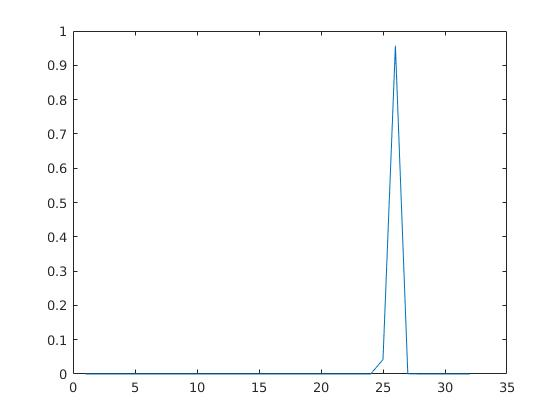
\includegraphics[height=120px]{../../results/gauss_f0.jpg}
\caption{$f_0$}
\end{figure}
}

\frame{
\frametitle{Exemple 1}
\begin{figure}[!h]
\centering
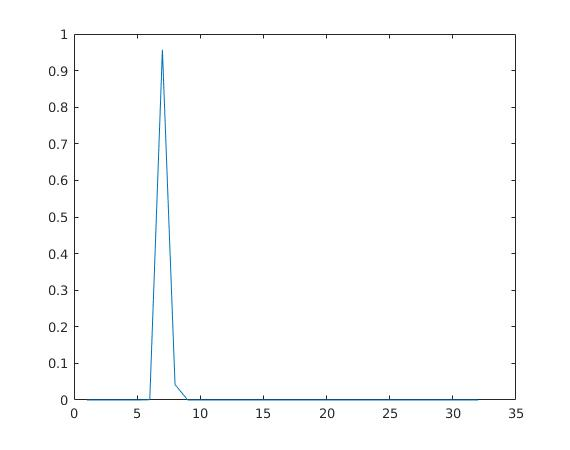
\includegraphics[height=120px]{../../results/gauss_f1.jpg}
\caption{$f_1$}
\end{figure}
}

\frame{
\frametitle{Exemple 1}
\begin{figure}[!h]
\centering
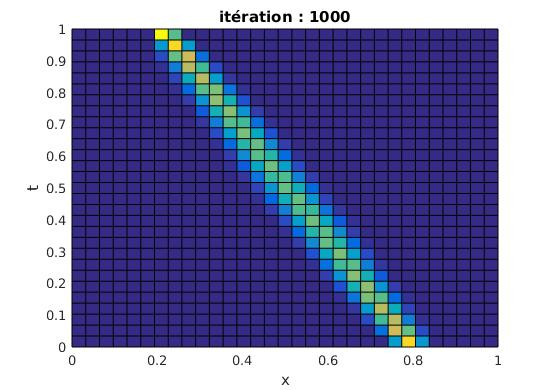
\includegraphics[height=120px]{../../results/gauss_transport.jpg}
\caption{Transport $f_0$ sur $f_1$}
\end{figure}
}

\subsection{Exemple 2}
\frame{
\frametitle{Exemple 2}
\begin{figure}[!h]
\centering
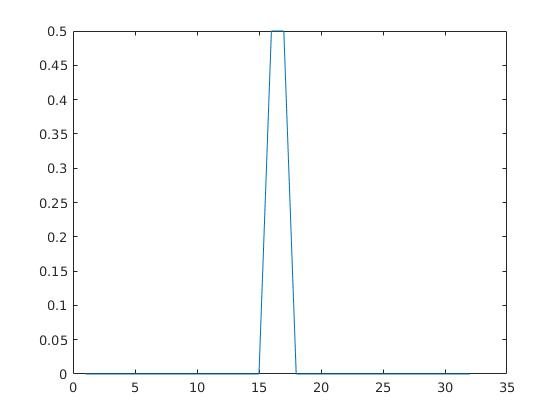
\includegraphics[height=120px]{../../results/gauss_mixture_f0.jpg}
\caption{$f_0$}
\end{figure}
}

\frame{
\frametitle{Exemple 2}
\begin{figure}[!h]
\centering
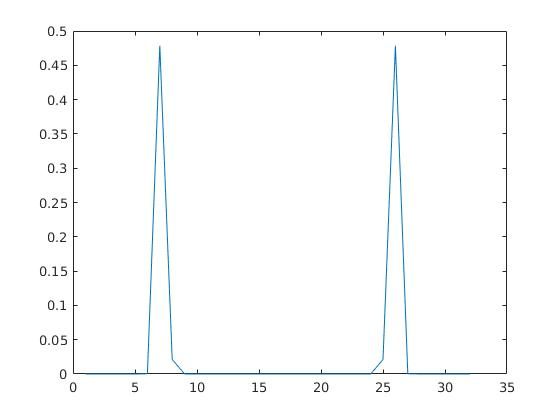
\includegraphics[height=120px]{../../results/gauss_mixture_f1.jpg}
\caption{$f_1$}
\end{figure}
}

\frame{
\frametitle{Exemple 2}
\begin{figure}[!h]
\centering
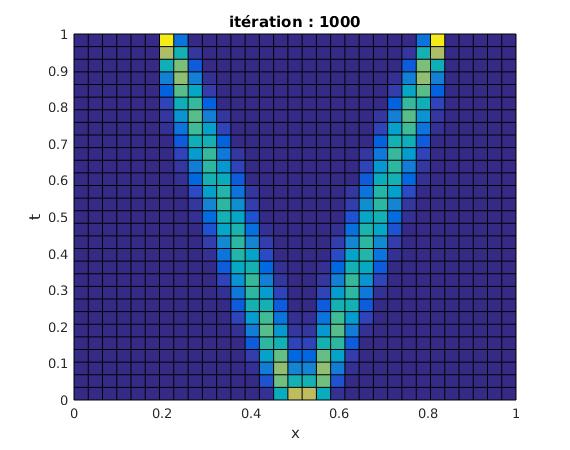
\includegraphics[height=120px]{../../results/gauss_mixture_transport.jpg}
\caption{Transport $f_0$ sur $f_1$}
\end{figure}
}

\subsection{Exemple 3}
\frame{
\frametitle{Exemple 3}
\begin{figure}[!h]
\centering
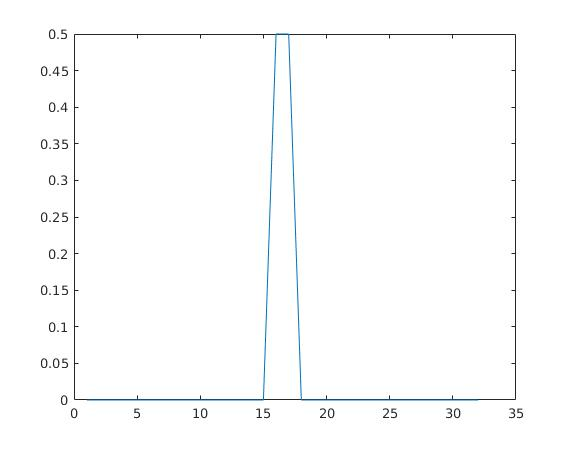
\includegraphics[height=120px]{../../results/gauss_sharp_f0.jpg}
\caption{$f_0$}
\end{figure}
}

\frame{
\frametitle{Exemple 3}
\begin{figure}[!h]
\centering
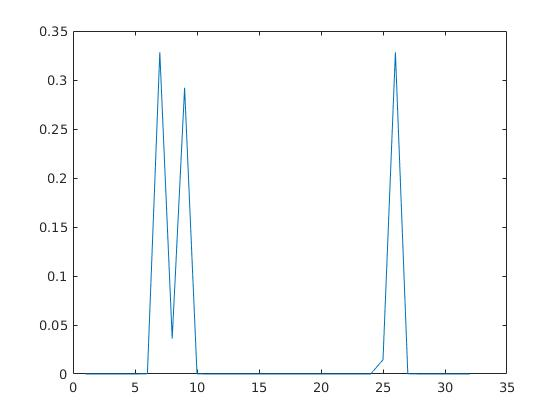
\includegraphics[height=120px]{../../results/gauss_sharp_f1.jpg}
\caption{$f_1$}
\end{figure}
}

\frame{
\frametitle{Exemple 3}
\begin{figure}[!h]
\centering
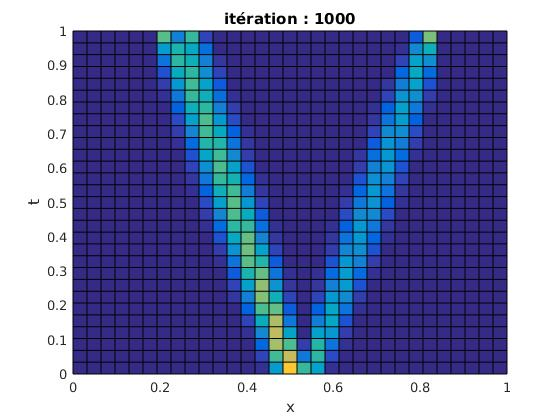
\includegraphics[height=120px]{../../results/gauss_sharp_transport.jpg}
\caption{Transport $f_0$ sur $f_1$}
\end{figure}
}




\end{document}

